\documentclass[../TDO3.tex]{subfiles}%

\begin{document}
\section[s]"1"{Constructions optiques de lentilles}

\enonce{%
	Construisez les images par la lentille des objets suivants. On donnera à chaque
	fois la \textbf{nature de l'objet et de l'image}.
}%

\QR{%
  \enonce{%
    \textbf{Pour une lentille convergente}
  }%
  \smallbreak
  \vspace{-15pt}
  \noindent
  \begin{isd}[interior hidden]
      \begin{enumerate}[leftmargin=20pt, label=\alph* --]
      \item Objet avant le foyer objet~;
      \item Objet sur le foyer objet~;
      \item Objet entre le foyer objet et la lentille~;
    \end{enumerate}
    \tcblower
      \begin{enumerate}[leftmargin=20pt, label=\alph* --, start=4]
      \item Objet après la lentille~;
      \item Faisceau parallèle à l'axe optique~;
      \item Rayon quelconque incliné par rapport à l'axe optique.
    \end{enumerate}
  \end{isd}
  \vspace{-15pt}
}{%
  \ifprof{%
      \vspace{-30pt}
  }%
  \begin{multicols}{2}
    \begin{enumerate}[leftmargin=20pt, label=\alph* --]
      \item ~\smallbreak
            \vspace*{-20pt}
            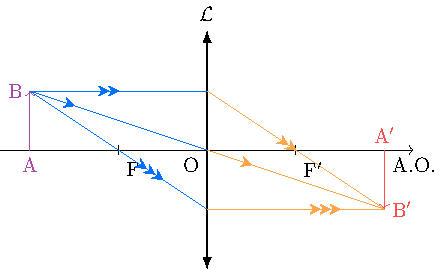
\includegraphics[width=\linewidth]{convAF}
            Ces rayons, issus d'un \xul{objet réel}, se croisent après la
            lentille~: on a un faisceau émergent \xul{convergent} qui
            donne une \xul{image réelle}.
      \item ~\smallbreak
            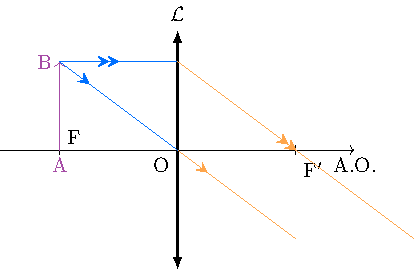
\includegraphics[width=\linewidth]{convBF}
            À partir d'un \xul{objet réel}, on obtient des rayons
            \xul{parallèles} qui donnent une \xul{image à l'infini}.
            \columnbreak
      \item ~\smallbreak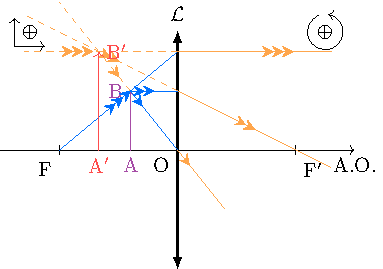
\includegraphics[width=\linewidth]{convCF}
            Ici, l'objet est \xul{réel} mais donne un faisceau émergent
            \xul{divergent}, donnant donc une image \xul{virtuelle}.
      \item ~\smallbreak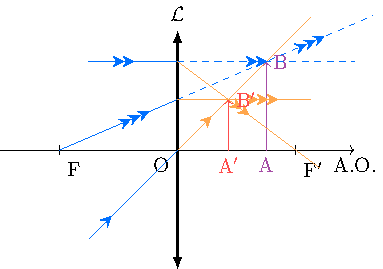
\includegraphics[width=\linewidth]{convDF}
            \xul{Objet virtuel}. Les rayons partant de la
            gauche passent par $B$, mais une fois arrivés à la lentille on les
            fait en pointillés, puisqu'ils sont virtuels. Le faisceau émergent
            est \xul{convergent}, donnant lieu à une \xul{image réelle}.
            \columnbreak
      \item ~\smallbreak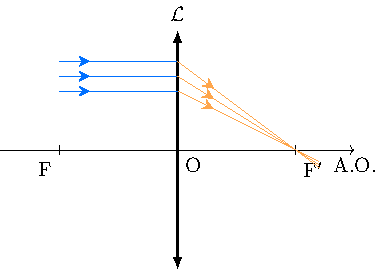
\includegraphics[width=\linewidth]{convHF}
            Ici, l'objet est \xul{réel} et donne un faisceau émergent
            \xul{convergent}, donnant donc une image \xul{réelle}.
      \item ~\smallbreak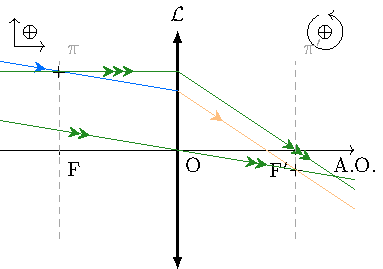
\includegraphics[width=\linewidth]{convQQE}
            On n'a qu'un seul rayon, donc pas d'intersection~: aucune idée de la
            nature de l'objet/image.
    \end{enumerate}
  \end{multicols}
}

\QR{%
	\textbf{Pour une lentille divergente}
  \smallbreak
  \vspace{-15pt}
  \noindent
  \begin{isd}[interior hidden]
      \begin{enumerate}[leftmargin=20pt, label=\alph* --]
		\item Objet avant le foyer image~;
		\item Objet entre le foyer objet et la lentille~;
		\item Objet sur le foyer objet~;
    \end{enumerate}
    \tcblower
      \begin{enumerate}[leftmargin=20pt, label=\alph* --, start=4]
		\item Objet après le foyer objet~;
		\item Faisceau parallèle à l'axe optique~;
		\item Rayon quelconque incliné par rapport à l'axe optique.
    \end{enumerate}
  \end{isd}
  \vspace{-15pt}
}{%
	\begin{multicols}{2}
    \ifprof{%
      \vspace{-30pt}
    }%
		\begin{enumerate}[leftmargin=20pt, label=\alph* --]
			\item ~
			      \smallbreak
			      \vspace*{-20pt}
			      \begin{center}
				      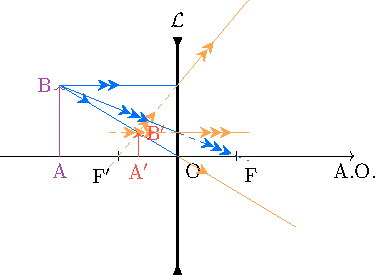
\includegraphics[width=\linewidth]{divAF}
			      \end{center}
			      Ces rayons, issus d'un \xul{objet réel}, se croisent avant la
			      lentille~: on a un faisceau émergent \xul{divergent} qui
			      donne une \xul{image virtuelle}.
            \ifprof{%
              \columnbreak
            }%
			\item ~\smallbreak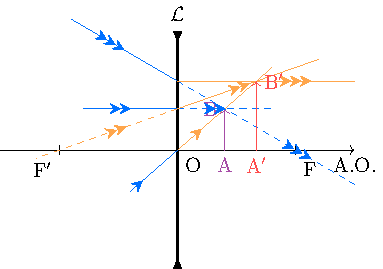
\includegraphics[width=\linewidth]{divBF}
			      À partir d'un \xul{objet virtuel}, on obtient des rayons
			      \xul{convergents} qui donnent une \xul{image réelle}.
              \columnbreak
			\item ~\smallbreak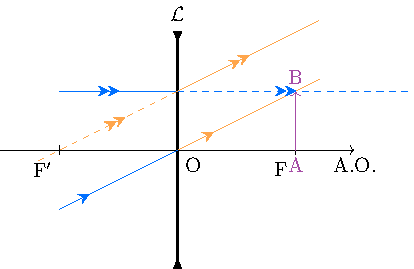
\includegraphics[width=\linewidth]{divCF}
			      Ici, l'objet est \xul{virtuel} et donne un faisceau émergent
			      \xul{parallèle}, donnant donc une image \xul{à l'infini}.
			\item ~\smallbreak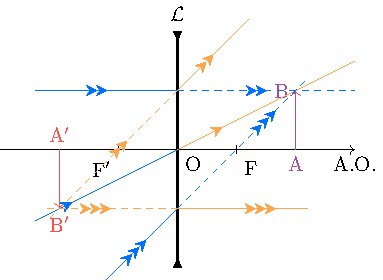
\includegraphics[width=\linewidth]{divDF}
			      On part d'un \xul{objet virtuel}. Le faisceau émergent est
			      \xul{divergent}, donnant lieu à une \xul{image virtuelle}.
			      \columnbreak
			\item ~\smallbreak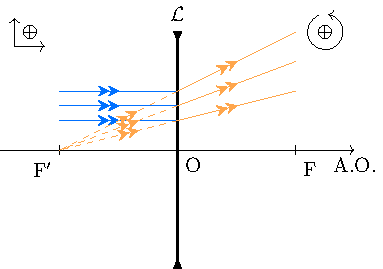
\includegraphics[width=\linewidth]{divHF}
			      Ici, l'objet est \xul{réel} et donne un faisceau émergent
			      \xul{divergent}, donnant donc une image \xul{virtuelle}.
			\item ~\smallbreak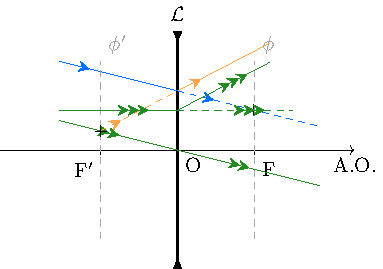
\includegraphics[width=\linewidth]{divQQE}
			      On n'a qu'un seul rayon, donc pas d'intersection~: aucune idée de la
			      nature de l'objet/image.
		\end{enumerate}
	\end{multicols}
}
\end{document}
